% 8 variables in here:
% u_1 = 0.0, h_1 = 10.0, U_1 = 0.0, H_1 = 10.0, u_2 = 0.0, h_2 = 10.0, U_2 = 0.0, H_2 = 10.0
%\renewcommand{\zoomfactor}{1.2}

\begin{figure}[ht]
  \centering
  \subfigure[Impulse error for varying point $p_1$] {
    \label{subfig:two-points-p1-height-momentum}
    % 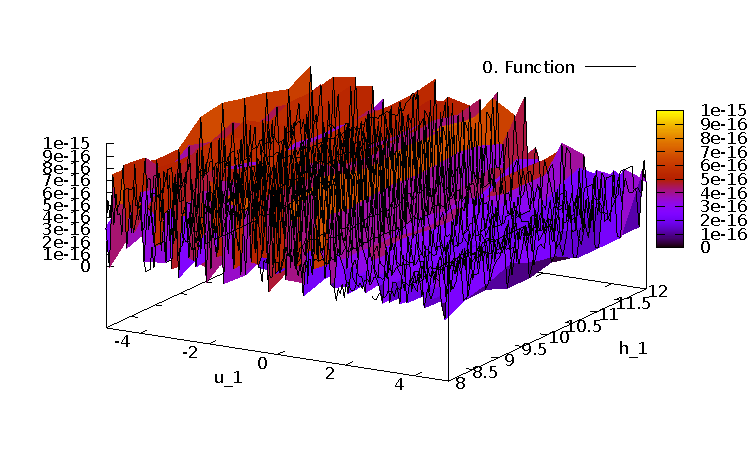
\includegraphics[scale=\zoomfactor]{{{2_punkte_alles_10_0/x_y_0.0_10.0_0.0_10.0_0.0_10.0f0}}}
    % \begin{tikzpicture}
    %   \node at (0,0) {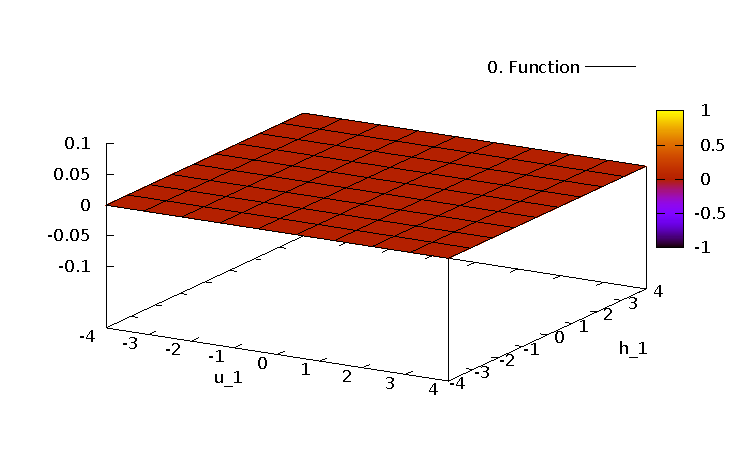
\includegraphics[scale=\zoomfactor]{zero_plots/u1h1}};
    %   \fill[white] (.8,1.2) rectangle (1.75,1.5);
    %   \node[align=right, text width=3cm] at (.2, 1.33) {\textsf{\tiny{Height error}}};
    % \end{tikzpicture}
    \begin{tikzpicture}
      \node at (0,0) {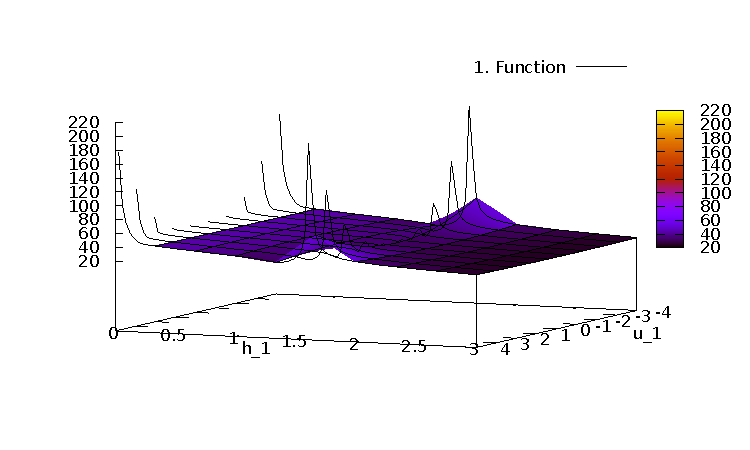
\includegraphics[scale=\zoomfactor]{{{2_punkte_alles_10_0/x_y_0.0_10.0_0.0_10.0_0.0_10.0f1}}}};
      \fill[white] (.8,1.2) rectangle (1.75,1.5);
      \node[align=right, text width=3cm] at (.2,1.33) {\textsf{\tiny{Impulse error}}};
    \end{tikzpicture}
  }
  \subfigure[Impulse error for varying point $p_2$] {
    \label{subfig:fixing-p2-in-first-example}
    % 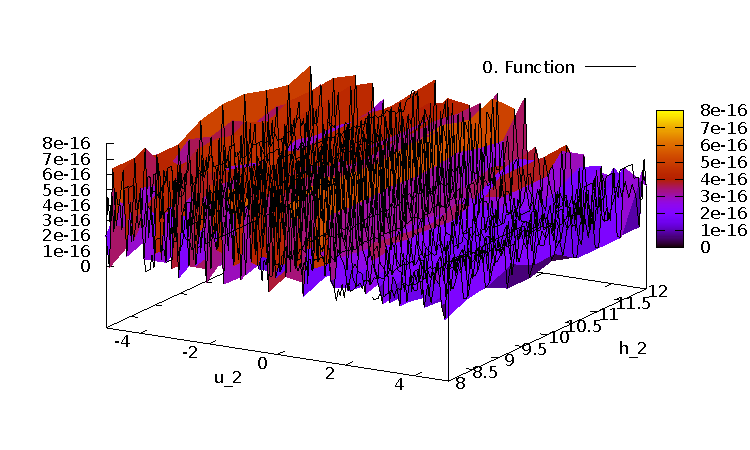
\includegraphics[scale=\zoomfactor]{{{2_punkte_alles_10_0/0.0_10.0_0.0_10.0_x_y_0.0_10.0f0}}}
    % \begin{tikzpicture}
    %   \node at (0,0) {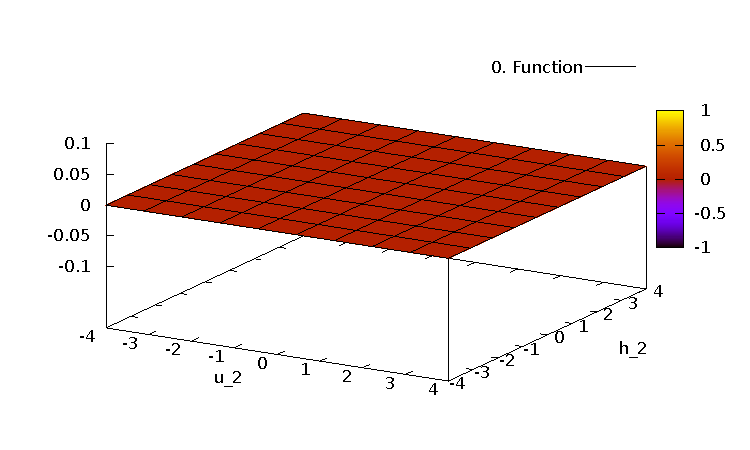
\includegraphics[scale=\zoomfactor]{zero_plots/u2h2}};
    %   \fill[white] (.8,1.2) rectangle (1.75,1.5);
    %   \node[align=right, text width=3cm] at (.2,1.33) {\textsf{\tiny{Height error}}};
    % \end{tikzpicture}
    \begin{tikzpicture}
      \node at (0,0) {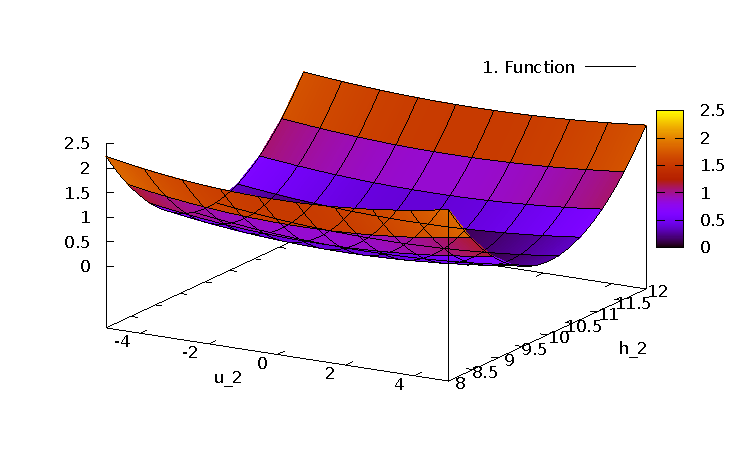
\includegraphics[scale=\zoomfactor]{{{2_punkte_alles_10_0/0.0_10.0_0.0_10.0_x_y_0.0_10.0f1}}}};
      \fill[white] (.8,1.2) rectangle (1.75,1.5);
      \node[align=right, text width=3cm] at (.2,1.33) {\textsf{\tiny{Impulse error}}};
    \end{tikzpicture}
  }
  \caption{Two points for each triangle. All support points have height 10 and impulse 0. $h$ ranges from 8 to 12, $u$ from -4 to 4. Note that the behaviour is completely symmetric. Varying the points of the other triangle (i.e. $p_1^R$ resp. $p_2^R$ yields the same plots.}
  \label{fig:two-points-all-the-same}
\end{figure}

%%% Local Variables:
%%% TeX-master: "../results.tex"
%%% End:

%%% Local Variables:
%%% TeX-master: "../results.tex"
%%% End:
